\documentclass[letterpaper]{article}
\usepackage{aaai19}
\usepackage{times} 
\usepackage{helvet}
\usepackage{courier} 
\usepackage[hyphens]{url}
\usepackage{graphicx}
\usepackage{float}
\urlstyle{rm}
\def\UrlFont{\rm}
\usepackage{graphicx}
\frenchspacing
\setlength{\pdfpagewidth}{8.5in}
\setlength{\pdfpageheight}{11in}
% custom packages%
\usepackage{amsmath}
\usepackage{enumitem}
\usepackage{subcaption}


\pdfinfo{
/Title (Detection of Price Manipulation in Cryptocurrencies)
/Author (Daniel Sapkota)
}

\setcounter{secnumdepth}{2} %May be changed to 1 or 2 if section numbers are desired.

\title{Detection of Price Manipulation in Cryptocurrencies}
\author{Daniel Sapkota}

\begin{document}

\maketitle

\begin{abstract}
    In this study, we use daily 
    OHLC and Margin position data from Bitfinex, and news posted on Reddit from November 10 2017
    to November 10 2019 to detect potential price manipulations in Bitcoin (BTC), Ethereum (ETH), 
    Ethereum Classic (ETC), ZCash (ZEC), and Litecoin (LTC). 
    We trained a random forest classifier 
    with a moving training test split starting from a training set of 200 days, and a test set 80 days. 
    We were able to detect potential manipulations at an AUC of 0.57, 0.72, 0.58, 0.58 and 0.54, respectively for BTC, ETH, ETC,
    ZEC and LTC.
    Backtesting the test set of 719 days in each coin
    with the same starting capital and a realistic fee of 0.1\% returned 
    828\%, 171\%, 169\%, 55.9\% and -23\% when buy and hold would have returned 
    -27\%, -86\%, 127\%, -50\% and 37.56\% each for ETH, ZEC, BTC, ETC and LTC.
     These strategies might be promising 
    for potential trading or law enforcement use. We explain the features used, 
    provide examples of the trading logic, and make our hypothesis.
\end{abstract}

\section{Introduction}
\label{sec:introduction}
\cite{griffin2019bitcoin,mirtaheri2019identifying,xu2019anatomy,gandal2018price,feder2018impact,li2019cryptocurrency}
have previously detected various forms of price manipulations within the cryptocurrency ecosystem.  
Even the CFTC has warned about cryptocurrency pump and dump schemes \cite{cftc_2018}. 
In Section \ref{sec:manipulations}, we detail and provide examples of various types of manipulations in the 
cryptocurrency ecosystem. Creating an approach that detects all of them is not possible. We create a
 hypothesis to generalize some price manipulations and attempt to detect them. We hypothesis the 
following:

\begin{itemize}
    \item Before a price altering news, Insiders, sometimes trade cryptocurrencies.
    \item Sometimes, the price goes up due to manipulations without any other significant event. 
    People who manipulate the price, buy it before the pump. 
    \item There are indicators, which can detect these events.
\end{itemize}

From here, we refer to the events we described in points 1 and 2 as Insider Trading. This is different than 
Insider Trading in the traditional sense as our definition also includes buying with an 
attempt to manipulate the price in the future as Insider Trading. \par

We determine our features based on previous studies and experiments. If our selected 
feature performs well in an unseen test set in a statistically significant way, price manipulation is likely. \par

In our manipulation detection algorithm, we created a condition to select eventful days based on news. 
We use Reddit to track news. Reddit is a discussion forum popular among cryptocurrency enthusiasts. Users 
 submit text and link posts to 
appropriate subreddits, and other users upvote/downvote it and add comments. Most of the discussion 
takes place in the comments section. The 
subreddits for Bitcoin, Ethereum, Litecoin, ZCash, and Ethereum Classic have 1.18M, 0.45M, 0.21M, 15k, and 25k 
subscribers as of November 10, 2019. The popularity of these subreddits between October 2017 and November 2019, 
is summarized in Table \ref{tab:Reddit-statistics}. 

\begin{table}[H]
    \begin{tabular}{|l|l|l|l|l|}
    \hline
    \textbf{Symbol} & \textbf{\begin{tabular}[c]{@{}l@{}}Avg Posts\\ per Day\end{tabular}} & \textbf{\begin{tabular}[c]{@{}l@{}}Avg Votes\\ per Post\end{tabular}} & \textbf{\begin{tabular}[c]{@{}l@{}}Avg News\\ per Day\end{tabular}} & \textbf{\begin{tabular}[c]{@{}l@{}}Avg Votes\\ per News\\ Post\end{tabular}} \\ \hline
    \textbf{BTC}    & 238.14                                                               & 30.45                                                                 & 29.01                                                               & 21.97                                                                        \\ \hline
    \textbf{ETH}    & 65.1                                                                 & 14.02                                                                 & 12.73                                                               & 17.23                                                                        \\ \hline
    \textbf{LTC}    & 16.52                                                                & 17.6                                                                  & 2.06                                                                & 20.25                                                                        \\ \hline
    \textbf{ETC}    & 7.99                                                                 & 3.69                                                                  & 1.36                                                                & 5.05                                                                         \\ \hline
    \textbf{ZEC}    & 3.77                                                                 & 6.68                                                                  & 0.6                                                                 & 8.72                                                                         \\ \hline
\end{tabular}
\caption{Reddit Statistics}
\label{tab:Reddit-statistics}
\end{table}

Reddit has an upvote and a downvote system. Posts 
with high votes go to the top, and more people see it. Among the submissions, we filtered out news 
by selecting 134 domains. The domains were chosen by manually looking at the 
most used domains in cryptocurrency-based subreddits. We selected traditional news sites, cryptocurrency-based news sites, and the official sites for most cryptocurrencies as news sites. The selected news domains 
is included in Appendix \ref{sec:news_sites}.
Table \ref{tab:Reddit-statistics} shows that these communities are popular enough for our 
purpose. \par

Bitcoin and other currencies can be traded in margin with leverage. Bitfinex provides leverage of 3.33 
\cite{Bitfinex}. These leveraged positions are referred to as longs and shorts. A long position profits when 
the price goes up, and short does when the price falls. Bitfinex provides the size of historical long and 
short positions opened during that time. We use that to calculate most of our features. \par

\section{Contributions of this study}
\label{sec:contributions}
\begin{itemize}
    \item We used news, chart and margin-based features to detect potential Insider Trading in a statistically signficant 
    way.
    \item We created a trading algorithm based on this, which showed a huge return. 
    \item We determine indicators from the Margin market, which can predict pumps.
\end{itemize}

\section{Literature Review}
\label{sec:literature_review}
We divide this section into two different subsections. First, we cite literature that explains the different types of 
manipulation that have been observed in cryptocurrencies. Then we explain approaches made at detecting them.

\subsection{Manipulations}
\label{sec:manipulations}
Since the beginning of financial markets, different types of manipulations have been observed 
\cite{markham2015law}. \cite{lin2016new} documented different strategies that have been used 
to manipulate the financial markets. The strategies include:

\begin{itemize}
    \item \textbf{Cornering and Sqeezing:} In this mechanism, one party obtains a significant portion of a financial 
    commodity and uses that to dictate the price \cite{markham2015law,lin2016new}. \cite{lin2016new} writes that 
    this mechanism is less common in liquid markets. In the past, single actors may have strategically made trades to cause 
    massive price changes, cornering, and squeezing the Bitcoin market \cite{griffin2019bitcoin}. 
    \item \textbf{Front Running:} In this type of manipulation, a broker performs trade before a market runner after 
    knowing their intention \cite{hazen1985law,markham2015law,lin2016new}. To our knowledge, this type of manipulation has not been 
    publicly documented in cryptocurrencies. However, exchanges have had issues. There have been “hacks” which 
    may not be a hack, exchanges have created trades without real money \cite{gandal2018price} and may still be 
    doing so \cite{griffin2019bitcoin}
    \item \textbf{Wash Trading:} Wash Trading is a form of manipulation where sham orders are made to create artificial volume and
    price \cite{teall2018financial}. Many cryptocurrency exchanges have meagre fees when trading at high volume. 
    OkEx, a cryptocurrency exchange, has confirmed having a Wash Trading problem \cite{baker_2019}
    \item \textbf{Spoofing:} Spoofing takes place when order is created without the intention of completing it. We have observed it many 
    times in different cryptocurrencies. Buy and Sell orders bigger than the total weekly volume have been documented. 
    They limit price growth/fall. \cite{unsafecoin_2016,bob_2017} 
    \item \textbf{Misinformation:} Fake news and social bots are distorting elections \cite{bessi2016social}. 
    They have been 
    used to manipulate stocks \cite{renault2017market}. 
    \cite{mirtaheri2019identifying} found an increase in bot activity in Social Media during price rises too.  
    \cite{zannettou2019let} found that state-sponsored Russian trolls discussed cryptocurrency in Reddit.
    \item \textbf{Insider Trading:} Company Insiders can have access to more information about the company than an outsider. If 
    they trade based on private information, they will have an advantage and are more likely to make profits/avoid 
    loss. Insider Trading is illegal in most commodities. On July 20, 2016, Ethereum was trading at 11.68\$. 
    On July 21, Coinbase, a US-based cryptocurrency exchange, added Ethereum. By July 22, it was trading at 15\$. 
    On May 3, 2017, Coinbase added Litecoin. On May 2, Litecoin traded at 15\$. By May 4, Litecoin was trading at 
    25\$. Insider trading was widely suspected during these instances. On December 19, 2017, Bitcoin Cash 
    was trading at 2000\$. On December 20, 2017, Coinbase added Bitcoin Cash. On the same day, Bitcoin Cash 
    traded at 4000\$. Coinbase is facing a class-action lawsuit over Insider Trading in this case. \cite{zhao_2018}
    \item \textbf{Pump and Dump:} During pump and dumps, a party acquires stock at cheap, artificially pump up the 
    price, and then sell it. \cite{mirtaheri2019identifying,xu2019anatomy} 
    examined Telegram Pump and Dump groups. Telegram Pump and Dump groups contain many members. Some groups 
    have a paid structure. A typical Telegram P\&D group works like this:

    \begin{itemize}
        \item The group admin buys a coin at cheap.
        \item The admin mentions the time he is going to pump a coin.
        \item At that time, the admin posts the name of the currency. In paid groups, paid members 
        see it first. As many people buy, the price goes up. After a while, other members 
        of the group get to see the message too. More people buy.
        \item Some people spread misinformation too. The success of the pump depends on the number of 
        people that buy the coin.
    \end{itemize}
 
    \cite{xu2019anatomy} used ML techniques from features derived from the Telegram data to detect 
    successful and unsuccessful attempts to manipulate large scale and medium scale cryptocurrencies. 
\end{itemize}

It is possible to perform many of these methods in combination.
For example, Cornering and Squeezing can be done to dump the price below a certain level. After accumulating 
an asset at cheap, Wash Trading can be done to create artificial volume. Spoofing orders can be made to create 
artifical demand. Then, misinformation can be spread. If all of these succeeds, the price goes up, and the pump and dump 
attempt completes.

\subsection{Detection}
From October 2013 to December 2013, the price of Bitcoin increased from 139\$ to over 1000\$. This
increase played a massive role in making Bitcoin more mainstream. During 
this time, Mt Gox was the leading Bitcoin exchange. Since then, Mt Gox has filed for Bankruptcy. After the bankruptcy
filing, \cite{gandal2018price} studied suspicious trades that took place in Mt Gox
during a ten-month period. \cite{gandal2018price} detected "Willy" and "Markus" bots that operated in Mt Gox
during this time. They found that price increased during 80\% of the day these bots operated. Price increased 
by 55\% on average when they did not operate. They conclude that these bots probably did not pay real money to perform the 
trades and were operated by the exchange itself. \par

From May 2017 to December 2017, the price of Bitcoin increased from 1300\$ to over 20000\$, creating a cryptocurrency
market cap of over 500 Billion \$. Although, there was a huge increase in people joining the exchanges, and 
Google Trends indicating an organic growth pattern, some form of manipulation was suspected. \cite{griffin2019bitcoin} 
conclude that a single actor likely drove the price by using a popular form of exchanging mechanism - USDT. They 
analyzed Bitcoin blockchain, USDT blockchain, and market data and found that less than 1\% of hours with heavy tether
transaction was associated with 50\% of the meteoric rise in Bitcoin. They show that this is not possible at random.
Although manipulation alone is not sufficient to create such growth, manipulation played a huge 
role in the timing of the rise. \par

In espionage, it is commonly known that strategically altering the key events can cause a huge change 
in the course of a nation when other factors are ripe for change. \cite{krafft2018experimental} performed small 
scale random trades in 
cryptocurrencies. They found that small buy actions caused a substantial increase in buy size activity that was 
hundereds of times the size of the interventions. If it scales up at this rate, given the right circumstance,
it explains how manipulations can create a big difference. \par

Studies have also found small actors manipulating the price of smaller coins. Manipulating small market cap 
seems easier and more common. \cite{xu2019anatomy} used data from 
Telegram channels to train a Neural Network that predicted a pump before it happens. By performing hypothetical
trade based on market features, they create a model with 0.96 AUC that can return over 60\% in 3 months.
Before them, \cite{li2019cryptocurrency} had also conducted a study using data from Telegram pump and dump groups. 
Recently \cite{mirtaheri2019identifying}
 created a model to detect the success of these pump attempts. They also study Twitter and detect a huge increase in 
the activity of Twitter Bots during manipulations. \par

There have been more studies of Insider Trading
outside cryptocurrencies. \cite{donoho2004early} used news and options based features to detect Insider Trading
in stocks. \cite{donoho2004early} created his features from call options and news, and detected 
Insider Trading.

\section{Approach}
\label{sec:approach}
\subsection{Data Collection}
\label{sec:data_collection}
First, we selected exchange to collect the data from. Bitfinex was chosen because it allows Margin Trading and has
 a strong connection with USDT, which has associated with some form of price manipulations. Although Bitfinex 
 is not the biggest exchange and conducts only a fraction of total trade, we assumed that the OHLC 
 data it provided was representative. Five currencies were selected for the sake of 
convinence. We selected the first five currencies that could be margin traded 
in Bitfinex. \par

We used the Bitfinex API to obtain the historical size of Long and Short positions. Then we obtained 
historic OHLC (Open, High, Low, Close) for the same dates using Bitfinex API. \par

There are many news sites and scraping data individually from all of them would be time-consuming. 
Additionally, it would be hard to separate the important from clickbait. So, we used Reddit as 
Reddit is popular and has a crowd filter mechanism. Reddit API does not provide historic subreddit submission data 
through an API. So, we used the Pushshift API to download historic submissions in the following subreddits:

\begin{itemize}
    \item /r/bitcoin for Bitcoin
    \item /r/ethereum for Ethereum
    \item /r/zec for ZCash
    \item /r/litecoin for Litecoin
    \item /r/ethereumclassic for Ethereum Classic
\end{itemize}

\subsection{Feature Calculation}
\label{sec:features}
After getting the required data, we calculated 59 features using the change in long and short positions 
and news. \par

\begin{table}[]
    \begin{tabular}{|l|l|l|l|}
    \hline
    \textbf{S.N.} & \textbf{Feature}                                                       & \textbf{Range} & \textbf{Meaning}                                                                                                                 \\ \hline
    1.            & total\_news                                                            & \begin{tabular}[c]{@{}l@{}}1D\\(24H)\end{tabular}               & \begin{tabular}[c]{@{}l@{}}Total Number of news \\ posted in Reddit \\ between 12 AM \\ to 12 AM\end{tabular}                                                                                            \\ \hline
    2.            & total\_sentiment                                                       & 1D              & \begin{tabular}[c]{@{}l@{}}Sum of the product of \\ Reddit score and \\ VADER \\ Sentiment\end{tabular}                                \\ \hline
    3.            & news\_dominance                                                        & 1D              & \begin{tabular}[c]{@{}l@{}}Total Score of news \\links divided by \\ total score of \\ non news links\end{tabular}                     \\ \hline
    4.            & \begin{tabular}[c]{@{}l@{}}normalized\_\\ mean\_sentiment\end{tabular} & 1D              & \begin{tabular}[c]{@{}l@{}}Mean of the score \\ times VADER \\ Sentiment\end{tabular}                                               \\ \hline
    5.            & mean\_sentiment                                                        & 1D              & \begin{tabular}[c]{@{}l@{}}Mean of VADER \\ Sentiment\end{tabular}                                                                                                          \\ \hline
    6.            & three\_day\_count                                                      &                    & \begin{tabular}[c]{@{}l@{}}Number of News \\ posted in the \\ last 3 days\end{tabular}                                                                                                \\ \hline
    7.            & thirty\_day\_count                                                     &                    & \begin{tabular}[c]{@{}l@{}}Number of News \\ posted in the last \\ 30 days\end{tabular}                                                                                               \\ \hline
    8.            & one\_thirty\_ratio                                                     &                    & \begin{tabular}[c]{@{}l@{}}Ratio of the number \\ of news in the \\ last day to the \\ number in the last \\ thirty days\end{tabular}    \\ \hline
    9.            & three\_thirty\_ratio                                                   &                    & \begin{tabular}[c]{@{}l@{}}Ratio of the number \\ of news in the \\ last 3 days to the \\ number in the last \\ thirty days\end{tabular} \\ \hline
    10.           & \begin{tabular}[c]{@{}l@{}}total\_\\sentiment\_\\mean\end{tabular}     & 20D              & \begin{tabular}[c]{@{}l@{}}Mean of the daily \\ sentiment for the \\ given time period \end{tabular}                                               \\ \hline
\end{tabular}
\caption{Reddit Based Features}
\label{tab:Reddit-features}
\end{table}

First, we filtered out link submission. We counted the number of links in a 24 hour range (starting at midnight) 
and filtered out news links.
Then we used VADER (Valence Aware 
Dictionary and sEntiment Reasoner) to calculate sentiment on the headlines instead of opening the link and scraping 
the news post. 
VADER is a rule-based 
sentiment classification designed for use in social media data. It returns a number between -1 and 1 from 
most negative to most positive \cite{hutto2014vader}.
VADER was chosen instead of SentiStrength, another popular sentiment analysis mechanism, because on 100 
random manual
 examinations, it performed better than SentiStrength. \par 

Then we converted all the Reddit and Bitfinex data to a daily range and calculated features detailed in 
Table \ref{tab:Reddit-features}, 
\ref{tab:donoho-features}, \ref{tab:price-features}. \par

\cite{donoho2004early} first used these features for Insider Trading detection in stocks using news and options data. 
Instead of options data, we used long-short data as the options market for cryptocurrency is relatively small. 
Features total\_news, three\_day\_count, thirty\_day\_count, 
one\_thirty\_ratio and three\_thirty\ ratio in Table 
\ref{tab:Reddit-features} were obtained from \cite{donoho2004early}. The other features in the table were manually
 tested and calculated. Most of the features on Table \ref{tab:donoho-features} were obtained from 
 \cite{donoho2004early} too. \par

\cite{xu2019anatomy} had used historic chart based features in their data when creating a model to
detect pumps from telegram data. Features 11 to 16 on table \ref{tab:price-features} were inspired by it.
\cite{xu2019anatomy} had used hourly data. However, we obtained higher accuracy with 
daily data. Features 7 to 10 were inspired by \cite{donoho2004early}

\begin{table}[]
    \begin{tabular}{|l|l|l|l|}
    \hline
    \textbf{S.N.} & \textbf{Feature}            & \textbf{Range}                                                        & \textbf{Meaning}                                                                                                                \\ \hline
    1.           & long              & 1D                 & \begin{tabular}[c]{@{}l@{}}Volume of total \\ Longs opened \\ during the end \\ of day\end{tabular}               \\ \hline
    2.           & short             & 1D                 & \begin{tabular}[c]{@{}l@{}}Volume of total \\ Shorts opened \\ during the end \\ of day\end{tabular}              \\ \hline
    3.            & \begin{tabular}[c]{@{}l@{}}longshort\_\\volume\end{tabular}           & 1D                                                                        & \begin{tabular}[c]{@{}l@{}}Sum of Total Longs \\ and Total Shorts\end{tabular}                                                                                             \\ \hline
    4.            & longshort\_ratio            & 1D                                                                        & \begin{tabular}[c]{@{}l@{}}Total longs divided \\ by total shorts.\end{tabular}                                                                                             \\ \hline
    5.            & mean\_volume                & \begin{tabular}[c]{@{}l@{}}20D:\\ Longs \\ and \\ Shorts\end{tabular} & \begin{tabular}[c]{@{}l@{}}Mean daily \\ volume during \\ 20D for\\ long and short\end{tabular}                                                                                                \\ \hline
    6.            & volume\_std                 & \begin{tabular}[c]{@{}l@{}}20D:\\ Longs \\ and \\ Shorts\end{tabular}                 & \begin{tabular}[c]{@{}l@{}}Standard Deviation \\ of the daily \\ long short volume \\ during the \\ 20D interval\end{tabular}                                                                                             \\ \hline
    7.           & times\_above                & \begin{tabular}[c]{@{}l@{}}20D:\\ Longs \\ and \\ Shorts\end{tabular}                 & \begin{tabular}[c]{@{}l@{}}How many times \\ above the 20D \\ average the volume \\ was\end{tabular}                             \\ \hline
    8.           & moving\_z\_score            & \begin{tabular}[c]{@{}l@{}}20D:\\ Longs \\ and \\ Shorts\end{tabular}                 & \begin{tabular}[c]{@{}l@{}}How many SD \\ above \\ 20D average\\ the volume was\end{tabular}                                     \\ \hline
    9.           & change                      & \begin{tabular}[c]{@{}l@{}}1D:\\ Longs \\ and \\ Shorts\end{tabular}                 & \begin{tabular}[c]{@{}l@{}}Percentage change \\ in volume \\ compared to the \\ previous day\end{tabular}                                  \\ \hline
    10.           & above\_average              & \begin{tabular}[c]{@{}l@{}}Daily:\\ Longs \\ and \\ Shorts\end{tabular}      & \begin{tabular}[c]{@{}l@{}}Number of times in \\ the last 5 days \\ that volume \\ exceeded \\ the 20 day \\ Moving Average\end{tabular} \\ \hline
    11.           & change\_avg                 & \begin{tabular}[c]{@{}l@{}}Daily:\\ Longs \\ and \\ Shorts \end{tabular}                                                              & \begin{tabular}[c]{@{}l@{}}Average change (9) \\ in volume  \end{tabular}                                                                                       \\ \hline
    12.          & \begin{tabular}[c]{@{}l@{}}today\_avg\_\\ comparision\end{tabular}     & \begin{tabular}[c]{@{}l@{}}Daily:\\ Longs \\ and \\ Shorts  \end{tabular}                                                             & \begin{tabular}[c]{@{}l@{}}Current Percentage \\ change divided by\\ the average change \\ over the last 20\\ intervals\end{tabular}  \\ \hline
    13.           & long\_short        & Daily                & \begin{tabular}[c]{@{}l@{}}Long Volume \\ divided \\ by the average\\ Short Volume of \\ the 3 biggest days\\ during the last \\ 20 days\end{tabular} \\ \hline
    14.           & short\_long        & Daily                & \begin{tabular}[c]{@{}l@{}}Short Volume \\ divided \\ by the average\\ Long Volume of \\ the 3 biggest days\\ during the last \\ 20 days\end{tabular} \\ \hline    
    \end{tabular}
\caption{Long Short Based Features}
\label{tab:donoho-features}
\end{table}

\begin{table}[]
    \begin{tabular}{|l|l|l|l|}
    \hline
    \textbf{S.N.} & \textbf{Feature}                                                    & \textbf{Range}                                                          & \textbf{Meaning}                                                                                                            \\ \hline
    1.            & Open                                                                & 1D                                                                          & \begin{tabular}[c]{@{}l@{}}Price of First \\ Trade during \\ the range\end{tabular}                                            \\ \hline
    2.            & High                                                                & 1D                                                                          & \begin{tabular}[c]{@{}l@{}}Price of biggest \\ Trade during \\ the day\end{tabular}                                          \\ \hline
    3.            & Low                                                                 & 1D                                                                          & \begin{tabular}[c]{@{}l@{}}Price of lowest \\ Trade during \\ the day\end{tabular}                                           \\ \hline
    4.            & Close                                                               & 1D                                                                          & \begin{tabular}[c]{@{}l@{}}Price of Last \\ Trade during \\ theday\end{tabular}                                              \\ \hline
    5.            & Volume                                                              & 1D                                                                          & \begin{tabular}[c]{@{}l@{}}Volume traded \\ in USDT\end{tabular}                                                                                                       \\ \hline
    6.            & Volume\_coin                                                        & 1D                                                                          & \begin{tabular}[c]{@{}l@{}}Volume traded \\ in currency\end{tabular}                                                                                                   \\ \hline
    7.            & Volatility                                                          & 5D                                                                       & \begin{tabular}[c]{@{}l@{}}Average of the \\ close values during \\ the last 5 days\end{tabular}                               \\ \hline
    8.            & volatility\_change                                                  & 5D                                                                       & \begin{tabular}[c]{@{}l@{}}Current volatility \\ divided by the\\ 5 day average\end{tabular}                              \\ \hline
    9.            & volume\_change                                                      & Daily                                                                            &  \begin{tabular}[c]{@{}l@{}}Current Volume \\ divided by the\\ 20 day average\end{tabular}                                                                                                                           \\ \hline
    10.           & two\_day\_change                                                    & Daily                                                                            &   \begin{tabular}[c]{@{}l@{}}Change in price \\ during the last\\ 2 days\end{tabular}                                                                                                                          \\ \hline
    11.           & return                                                              & \begin{tabular}[c]{@{}l@{}}1D,2D,3D\end{tabular} & \begin{tabular}[c]{@{}l@{}}Log return of \\ the change in close\\ price during \\ the interval\end{tabular} \\ \hline
    12.           & volume\_from                                                        & \begin{tabular}[c]{@{}l@{}}1D,2D,3D\end{tabular} & \begin{tabular}[c]{@{}l@{}}Sum of the \\ volume in USDT in\\ the given interval\end{tabular}                                   \\ \hline
    13.           & volume\_to                                                          & \begin{tabular}[c]{@{}l@{}}1D,2D,3D\end{tabular} & \begin{tabular}[c]{@{}l@{}}Sum of the \\ volume in coin in\\ the given interval\end{tabular}                                   \\ \hline
    14.           & return\_volatility                                                  & \begin{tabular}[c]{@{}l@{}}1D,2D,3D\end{tabular} & \begin{tabular}[c]{@{}l@{}}Std of the \\ calculated log \\ return during the \\ given timeframe\end{tabular}   \\ \hline
    15.           & \begin{tabular}[c]{@{}l@{}}volume\_from\_\\ volatility\end{tabular} & \begin{tabular}[c]{@{}l@{}}1D,2D,3D\end{tabular} & \begin{tabular}[c]{@{}l@{}}Std of the \\ volume in USDT \\ during the given \\ timeframe\end{tabular}                                 \\ \hline
    16.           & \begin{tabular}[c]{@{}l@{}}volume\_to\_\\ volatility\end{tabular}   & \begin{tabular}[c]{@{}l@{}}1D,2D,3D\end{tabular} & \begin{tabular}[c]{@{}l@{}}Std of the \\ volume in coin \\ during the given \\ timeframe\end{tabular}                                  \\ \hline
\end{tabular}
\caption{Price Based Features}
\label{tab:price-features}
\end{table}

\subsection{Creating Classification}
\label{sec:creating_y}
Random Forest, a Supervised Machine Learning technique, is used to create the ML model. It requires 
supervised classification of data before training. We name this classification column y. From manual 
inspection, we created a logic to determine huge rises.
To do that, we initially set y to 0. If the predetermined conditions were met, the value of that day and the 14 
days before it is set to 1. We number 14 days before a big rise as 1 too because 
we had hypothesized that buying takes place slowly before a huge rise, \cite{donoho2004early} had 
success using it, and we wanted to prevent a heavily imbalanced dataset. The predetermined 
conditions were:
\begin{itemize}
    \item The product of total votes and the sentiment of the news post is greater than 10, or
    the number of news posted that day is greater than or equal to 5 percent of the total posts in the last 
    30 days. This was done because \cite{donoho2004early} had used this in a similar system, it was congurent
    with our logic and, later we found out that using this logic had increased the accuracy, AUC, and profit in our 
    model.
    \item Tomorrow's price is at least 5 percent greater than today.
    \item Price 5 days later is at least 5 percent greater than today. 
    \item The percentage change in price over the last 15 days is positive.
\end{itemize}
    
This logic classified the major pumps in all five currency fairly well. A figure representing the classified 
points is included in Appendix \ref{sec:classification_y}

\subsection{Machine Learning Model}
\label{sec:model_creation}
In supervised Machine Learning, we divide data into training and test set. The training set is used to train the 
algorithm. The test set is used to test how it works. There are many approaches to create a training and a test set.
We had three options:
\begin{itemize}
    \item \textbf{Train Test Split:}Select the first n\% of the data as the training set and use the remaining data as 
   the test set. 
    \item \textbf{K-Fold Cross Validation:} Divide the data into k random folds. Train different models with 
    a different test set in each model.
    \item \textbf{Walk Forward Validation:} Start with n days as the training set and y days as the test set.
    Iterate till the end by increasing the size of the training set by y until the end is reached.
\end{itemize}
   
We chose the walk-forward validation as it was robust and provided us with a huge test set that could be 
tested in different market periods. 
We started with the first 200 days as training set and 80 days after it as the test
 set. Then, we increased the size 
 of the training set by 80 days i.e., 280 days with the next 80 days as a test set.
 We repeated this till we reached the end. This way, we had 
 access to a long test set.
 In each step, we standardized the training and the test set by subtracting 
 it with the mean of the training set and 
dividing by the standard deviation of the training set. The training set's mean was used to prevent 
any leakage of future data in the test set. \par 

We trained a different random forest classifier using 100 estimators for each coin.

\subsection{Backtesting}
\label{sec:backtest}
After creating the models, the model's prediction on the test set was used to perform backtesting with a realistic
 0.1\% fee. We started with a capital of 10000\$ for each coin. The trading logic for each coin was:
\bigskip\bigskip



\noindent If no position is currently open in that coin:
 \begin{itemize}
 \item Open a position with 95\% of the allocated capital for that coin if the prediction is 1.
 \item Do not do anything if the prediction is 0
 \end{itemize}
 \bigskip

\noindent If a position is currently open, we first set n to 4. Then:
\begin{itemize}
 \item Hold for n days and sell all open position if prediction changes to 0 from 1
 \item Set n to 4 days if the prediction is 1
\end{itemize}

\bigskip

\section{Explanations and Result}
\label{sec:result}

The obtained result is summarized in Table \ref{tab:result-metrics}. 

\begin{table}[H]
    \begin{tabular}{|l|l|l|l|l|}
    \hline
    \textbf{Symbol} & \textbf{AUC} & \textbf{Accuracy} & \textbf{\begin{tabular}[c]{@{}l@{}}Hold \\ Return \\ (\%)\end{tabular}} & \textbf{\begin{tabular}[c]{@{}l@{}}Algorithm \\ Return (\%)\end{tabular}} \\ \hline
    \textbf{ETH}    & 0.72         & 0.82             & -27.38                                                                  & 828.06                                                                    \\ \hline
    \textbf{BTC}    & 0.57         & 0.63              & 127.55                                                                  & 169.17                                                                    \\ \hline
    \textbf{ZEC}    & 0.58         & 0.86              & -86.75                                                                  & 171.31                                                                    \\ \hline
    \textbf{ETC}    & 0.58          & 0.87              & -50.86                                                                  & 55.9                                                                         \\ \hline
    \textbf{LTC}    & 0.44         & 0.81               & 37.56                                                                   & -23.18                                                                    \\ \hline
\end{tabular}
\caption{Result Metrics}
\label{tab:result-metrics}
\end{table}

Area Under the Curve (AUC) and the Accuracy of the predictions in the test set is provided in Table \ref{tab:result-metrics}. 
AUC is considered a better metric in the ML literature than accuracy in an unbalanced dataset like this. 
High accuracy can be obtained by predicting in the same direction. Our task is price prediction. 
So although our AUC is not extremely high, it is fairly high 
for this task. \par


\begin{table}[H]
    \begin{tabular}{|l|l|l|l|l|l|}
    \hline
    \multicolumn{1}{|c|}{\textbf{Symbol}} & \multicolumn{1}{c|}{\textbf{\begin{tabular}[c]{@{}c@{}}Total \\ Positions\end{tabular}}} & \multicolumn{1}{c|}{\textbf{\begin{tabular}[c]{@{}c@{}}Total\\ Profit\end{tabular}}} & \multicolumn{1}{c|}{\textbf{\begin{tabular}[c]{@{}c@{}}Total\\ Lost\end{tabular}}} & \multicolumn{1}{c|}{\textbf{\begin{tabular}[c]{@{}c@{}}Avg\\Profit\end{tabular}}} & \multicolumn{1}{c|}{\textbf{\begin{tabular}[c]{@{}c@{}}Avg \\ Loss\end{tabular}}} \\ \hline
    ETH                                   & 20                                                                                       & 14                                                                                & 6                                                                                  & 8279.57                                                                         & -5517.95                                                                          \\ \hline
    ZEC                                   & 8                                                                                        & 8                                                                                 & 0                                                                                  & 2141.36                                                                         & 0                                                                                 \\ \hline
    BTC                                   & 28                                                                                       & 17                                                                                & 11                                                                                 & 1695.1                                                                          & -1081.76                                                                          \\ \hline
    ETC                                   & 6                                                                                        & 4                                                                                 & 2                                                                                  & 1471.83                                                                         & -148.7                                                                            \\ \hline
    LTC                                   & 14                                                                                       & 6                                                                                 & 8                                                                                  & 1111.42                                                                         & -1123.34                                                                          \\ \hline
\end{tabular}
\caption{Position Details}
\label{tab:pos-detail}
\end{table}


Table \ref{tab:pos-detail} shows that the algorithm opened few positions. Nevertheless, the return is enormous.
A successful trade returned at least 1000\$. The number of successful trades was higher than losing one in all 
currencies except Litecoin. The average profit during a success was also bigger than the average 
loss in all of these currencies, excluding Litecoin.

\begin{table}[H]
\begin{tabular}{|l|l|l|l|l|}
    \hline
    \textbf{Symbol} & \textbf{\begin{tabular}[c]{@{}l@{}}one \\ actual\end{tabular}} & \textbf{\begin{tabular}[c]{@{}l@{}}one \\ predicted\end{tabular}} & \textbf{\begin{tabular}[c]{@{}l@{}}zero \\ actual\end{tabular}} & \textbf{\begin{tabular}[c]{@{}l@{}}zero \\ predicted\end{tabular}} \\ \hline
    ETH             & 178                                                            & 144                                                               & 542                                                             & 576                                                                \\ \hline
    ZEC             & 90                                                             & 44                                                                & 590                                                             & 636                                                                \\ \hline
    BTC             & 222                                                            & 229                                                               & 498                                                             & 491                                                                \\ \hline
    ETC             & 97                                                             & 31                                                                & 623                                                             & 689                                                                \\ \hline
    LTC             & 99                                                             & 68                                                                & 621                                                             & 652                                                                \\ \hline
\end{tabular}
\caption{Output comparision}
\label{tab:output-comparision}
\end{table}
The number of  predicted and actual ones and zeros is included in Table \ref{tab:output-comparision}. 
The number is quite similar. 

The backtest diagram is included in Appendix \ref{sec:backtest_chart}. When a position is opened, there 
is a green mark. When it is closed, there is a red mark. Our model predicted most of the huge price increases in Ethereum,
ZCash, Ethereum Classic and Bitcoin. It did not perform as well for Litecoin. \par

\begin{figure}[H]
    \centering
    \captionsetup{justification=centering}

    \begin{subfigure}[b]{0.4\linewidth}
      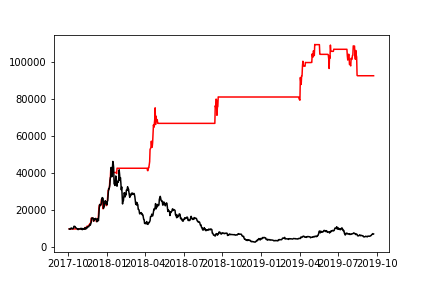
\includegraphics[width=\linewidth]{images/portfolio/ETH.png}
      \caption{ETH}
    \end{subfigure}
    \begin{subfigure}[b]{0.4\linewidth}
      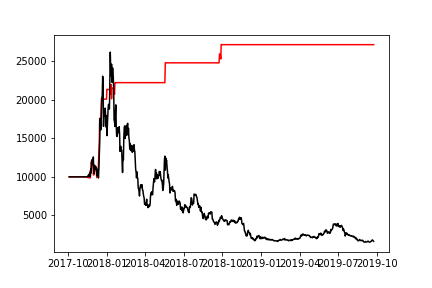
\includegraphics[width=\linewidth]{images/portfolio/ZEC.png}
      \caption{ZEC}
    \end{subfigure}
    \begin{subfigure}[b]{0.4\linewidth}
        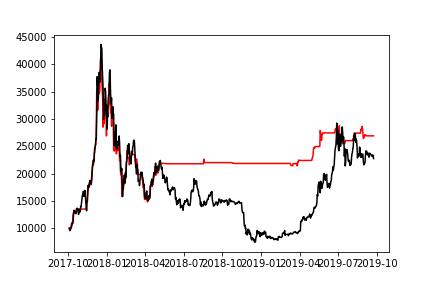
\includegraphics[width=\linewidth]{images/portfolio/BTC.png}
        \caption{BTC}
      \end{subfigure}
      \begin{subfigure}[b]{0.4\linewidth}
        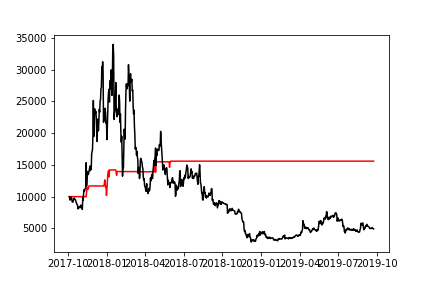
\includegraphics[width=\linewidth]{images/portfolio/ETC.png}
        \caption{ETC}
    \end{subfigure}
    \begin{subfigure}[b]{0.4\linewidth}
        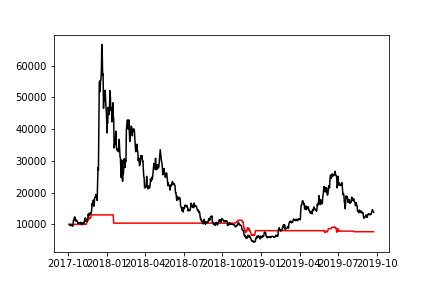
\includegraphics[width=\linewidth]{images/portfolio/LTC.png}
        \caption{LTC}
    \end{subfigure}

    \caption{Our Algorithm VS holding}
    \label{fig:algo_vs_hold}
\end{figure}

We started with 10,000\$ in each coin. The movement of the portfolio for each coin is in Figure \ref{fig:algo_vs_hold}.
The black line represents and holding portfolio while the red line shows our algorithm. 
We can see in the Figures that the portfolio value increases most of the time when the value of the coin increases.
However, it does not fall when the price falls. A trading model may be able to increase profit by predicting the 
falls and performing shorts. \par

\section{Model Examination}
\label{sec:model_examination}

ML models are frequently left black box.
In this section, we try to understand why our algorithm brought and sold the way it did. We analyzed the
random forest classifier to find out the most significant features. The feature importance function in scikit learn
was used for this purpose. The five most important features, contributing about 25\% of each coin is in Table 
\ref{tab:important-features}. 

\begin{table}[H]
    \begin{tabular}{|l|l|l|l|l|l|}
    \hline
    \textbf{feature}                                                    & \textbf{ETH} & \textbf{BTC} & \textbf{ZEC} & \textbf{ETC} & \textbf{LTC} \\ \hline
    \begin{tabular}[c]{@{}l@{}}20D\_short\_\\ volume\_mean\end{tabular} & 0.11         & 0.05         & 0.04         & 0.02         & 0.08         \\ \hline
    \begin{tabular}[c]{@{}l@{}}20D\_long\_\\ volume\_mean\end{tabular}  & 0.03         & 0.06         & 0.08         & 0.03         & 0.04         \\ \hline
    \begin{tabular}[c]{@{}l@{}}20D\_long\_\\ volume\_std\end{tabular}   & 0.04         & 0.05         & 0.04         & 0.03         & 0.08         \\ \hline
    short                                                               & 0.03         & 0.05         & 0.07         & 0.01         & 0.04         \\ \hline
    long                                                                & 0.03         & 0.04         & 0.04         & 0.05         & 0.03         \\ \hline
\end{tabular}
\caption{Important Features}
\label{tab:important-features}
\end{table}


All features and their importance in each coin is in Appendix \ref{sec:feature_strength}. 
These tables show that features derived from long and short were most powerful.
They were responsible for nearly 50\% of the model in all coins. We analyze 
some trades our mode primarily made based on these feature this section. \par


Price change depends on many factors. In this study, we selected some and found that they could predict 
some price increases correctly. In this section, for intuition, we selected only two features. 
We only perform a surface examination and do not see how it correlates with other features. 

\subsection{Ethereum- November 2017 to March 2018}
\label{sec:jan_ethereum}
In Appendix \ref{sec:backtest_chart}, we can see that the price of ETH was 313\$ on November 15, 2017. By January 
14 it had gone up to 1257\$. Our algorithm had performed a near-perfect trade by buy at 313\$ and 
selling at 1257\$. 

\begin{figure}[h!]
    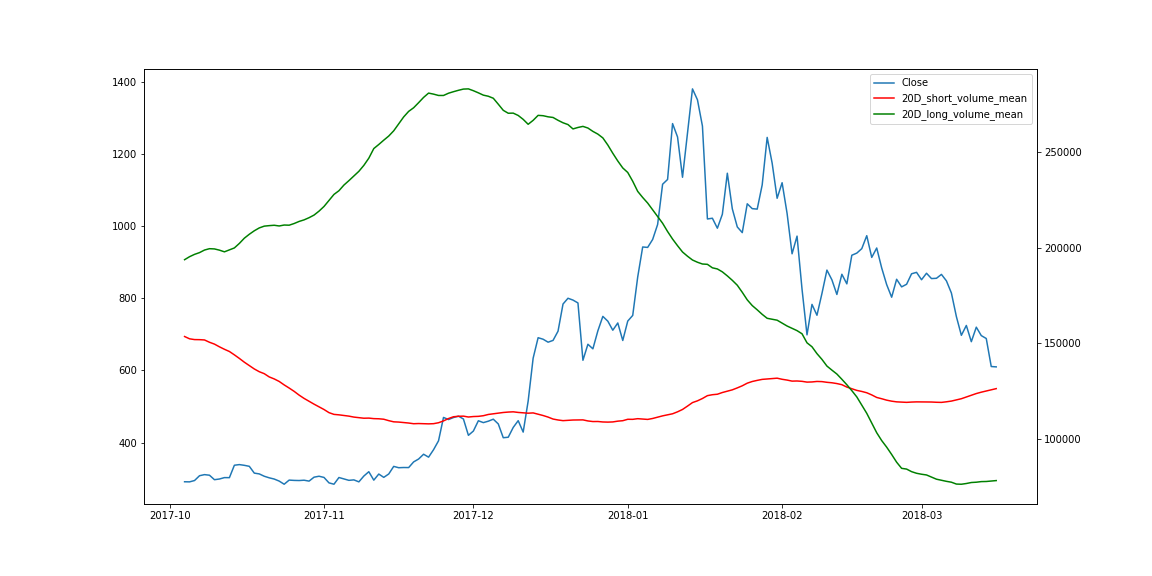
\includegraphics[width=\linewidth]{images/case1.png}
    \caption{Ethereum around January 2018}
    \label{fig:eth_jan}
\end{figure}

Figure \ref{fig:eth_jan} shown above can be zoomed for detail. In the figure, the blue line represents the daily
close price of Ethereum. Its axis is on the left. On the right, there is another axis for the 20-day short volume 
mean, and the 20-day long volume mean. The long volume is in green while the short volume is in red. In the 
figure, we can see the Long volume rises and short volume falls before the price increase in December 2017.
Then the long volume remains up for some time. The long volume starts falling in January 2018, before the fall in price. The 
short volume also increases before the fall. As these are the most powerful feature, and most other features 
also derived from long and short, we can hypothesize that our 
algorithm was triggered by the changes in it. The decision turned out to be correct. 

\subsection{April 2018 - Ethereum}
\label{sec:april_ethereum}
On April 10, our algorithm brought Ethereum at 400\$. On April 26, it sold it at 702\$.

\begin{figure}[h!]
    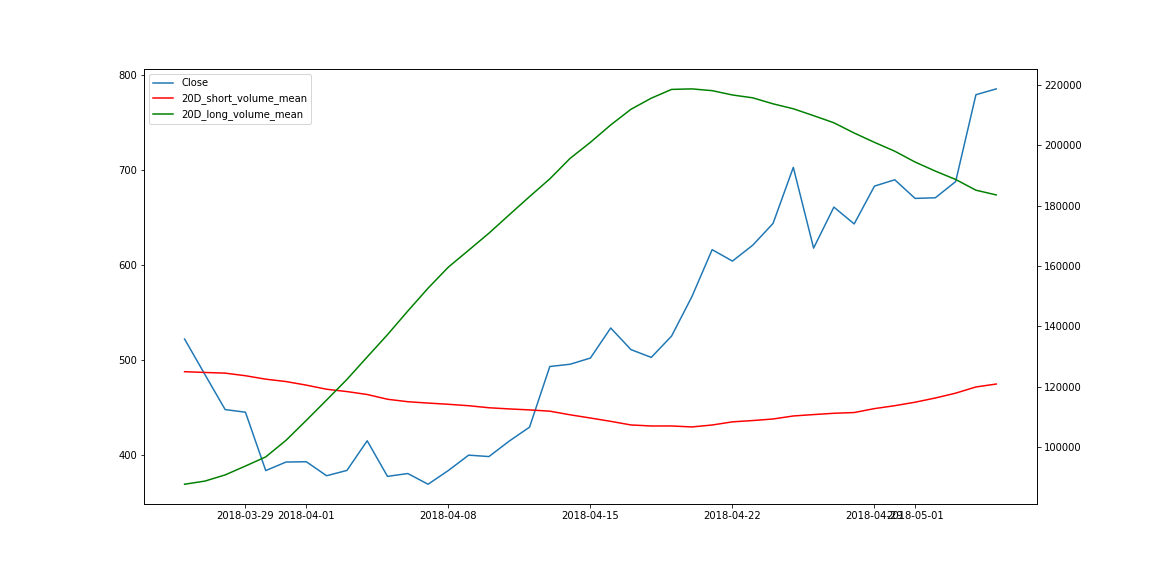
\includegraphics[width=\linewidth]{images/case2.png}
    \caption{Ethereum around April 2018}
    \label{fig:eth_april}
\end{figure}

We draw a similar figure and have a similar observation in Figure \ref{fig:eth_april}. The 20 day long rises. The 
20D short average falls. Then the price increases. After April 20, the long average starts falling, and shorts 
start rising. The price then follows the long average and goes down.

\subsection{January 2017 - ZCash}
\label{sec:jan_zcash}
On December 13, 2017, our model brought ZCash at 317\$. On December 20, it sold it at 600\$.

\begin{figure}[h!]
    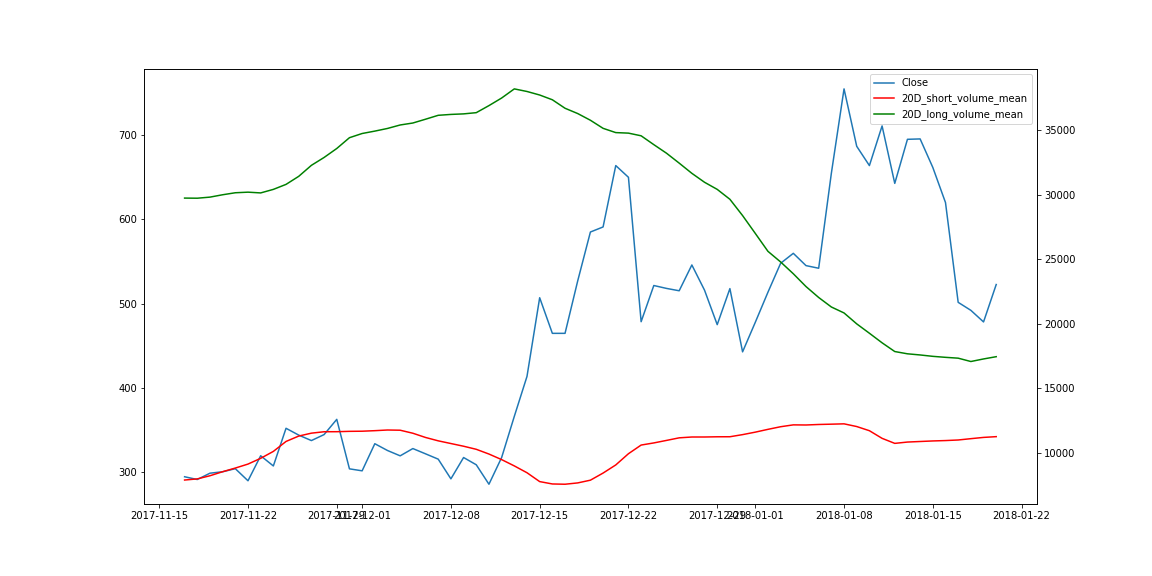
\includegraphics[width=\linewidth]{images/case3.png}
    \caption{ZCash around January 2017}
    \label{fig:zec_jan}
\end{figure}

Figure \ref{fig:zec_jan} shows a similar case for ZCash. The 20 day long rises, then the price. 

\section{Conclusion}
\label{sec:conclusion}
We started the study, assuming that Insider Trading takes place based on previous literature. 
We used features that are possibly indicative of Insider Trading 
and created an ML model. The model performed much better than holding in the test set. \par

To learn if our success can happen due to chance, 
we selected 59 random features between 1 and -1 from a uniform distribution and created a 
Random Forest classifier, based on the same split mechanism as we did for our algorithm.
We ran the simulation for 3000 iterations. None of the 3000 models performed 
as good as our algorithm. We assumed a starting capital of 10000\$ for each coin and added the final 
value for each to calculate the total return. Using this mechanism, our algorithm had returned 
240\%. In 3000 iterations, the best random 
model returned 100\%. The average portfolio value at the end was 49034\$, slightly less than the starting price. 
The standard deviation was 7150\$. 
The sum of the 5 AUC our model predicted was 2.99. The best random model had 2.64.
 \par

 This shows that this behaviour is extremely unlikely on random. Our features were responsible for the correct 
 detection. Thus, Insider Trading probably 
takes place and can be detected using public data. Although Insider Trading cannot exactly be proved with 
100\% certainty by 
this mechanism, we show that it is likely the case.

\section{Further Work}
\label{sec:further_work}
In our study, we did not use all possible forms of data available to us. 
We did not use data from the blockchain. In the future, 
clustering techniques can be used to cluster addresses and 
watch the flow of transactions. Features can be created from it. \par

We used Reddit data in this work. \cite{mirtaheri2019identifying} showed that bots are used during 
pumps. We can use bot detection techniques on Reddit and on Twitter to correlate the 
 bots with pump attempts. \cite{xu2019anatomy,mirtaheri2019identifying} had 
success with Telegram data. A comprehensive model can have a place for them too.\par

There may be a place for integration of order book data, too, in a sophisticated system. However, integrating 
all of them may be a very complicated task.\par

Finally, different groups may have caused different pumps. We may be able to use techniques
from cyber forensics and unsupervised machine learning to find types of groups and find a signature. 
 Research in this direction will be helpful for Law Enforcement 
too.
*
\bibliographystyle{aaai}
\bibliography{references}

\newpage
\onecolumn

\section{Appendix}
\label{sec:appendix}

\subsection{News Sites}
\label{sec:news_sites}

\begin{table}[H]
    \begin{tabular}{|l|l|l|l|l|}
    \hline
    coindesk.com        & marketwatch.com            & 0xproject.com          & allcryptocurrencies.news   & tezos.foundation   \\ \hline
    medium.com          & theguardian.com            & discord.gg             & crypto-lines.com           & tezosfoundation.ch \\ \hline
    cointelegraph.com   & coinbase.com               & coinwhalenews.com      & iotahispano.com            &                    \\ \hline
    bitcoin.com         & wired.com                  & cryptotown.io          & iota-news.com              &                    \\ \hline
    cryptocoinsnews.com & bbc.co.uk                  & investinblockchain.com & ethereumworldnews.com      &                    \\ \hline
    newsbtc.com         & cryptobrowser.site         & publish0x.com          & oracletimes.com            &                    \\ \hline
    bloomberg.com       & vice.com                   & cointopper.com         & litecoin.com               &                    \\ \hline
    cnbc.com            & insidebitcoins.com         & etherscan.io           & monerobase.com             &                    \\ \hline
    bitcoinmagazine.com & ft.com                     & coingeek.com           & moneroblocks.info          &                    \\ \hline
    forbes.com          & themerkle.com              & craigwright.net        & ripple.com                 &                    \\ \hline
    bitcoinist.com      & fortune.com                & coinblockdesk.com      & ripplenews.tech            &                    \\ \hline
    bitcoinist.net      & tumblr.com                 & coingecko.com          & omisego.network            &                    \\ \hline
    github.com          & coinspeaker.com            & yours.org              & omise.co                   &                    \\ \hline
    zerohedge.com       & coinjournal.net            & cryptodaily.co.uk      & coinspot.com.au            &                    \\ \hline
    ambcrypto.com       & beincrypto.com             & coinidol.com           & coincodex.com              &                    \\ \hline
    businessinsider.com & seekingalpha.com           & businessdigit.com      & smartlands.io              &                    \\ \hline
    bitcoinfeeds.com    & arstechnica.com            & cryptolinenews.com     & todaysgazette.com          &                    \\ \hline
    steemit.com         & rt.com                     & blockchain.info        & samcrypto.com              &                    \\ \hline
    wsj.com             & wikipedia.org              & coin.dance             & linkedin.com               &                    \\ \hline
    newsforyou.today    & theverge.com               & linuxfoundation.org    & discussions.app            &                    \\ \hline
    bitcoinvox.com      & btcfeed.net                & dashforcenews.com      & theeoswriter.io            &                    \\ \hline
    nytimes.com         & tradingview.com            & dashnews.org           & eoswriter.io               &                    \\ \hline
    yahoo.com           & bbc.com                    & dash.org               & theaccountingblockchain.io &                    \\ \hline
    reuters.com         & ibtimes.co.uk              & dashcentral.org        & eosauthority.com           &                    \\ \hline
    coinfox.info        & bitguru.co.uk              & dashpaymagazine.com    & neonbeginner.com           &                    \\ \hline
    toshitimes.com      & the-blockchain-journal.com & cryptobriefing.com     & neonewstoday.com           &                    \\ \hline
    bravenewcoin.com    & qz.com                     & financemagnates.com    & neo.org                    &                    \\ \hline
    techcrunch.com      & washingtonpost.com         & thedashtimes.com       & z.cash                     &                    \\ \hline
    ccn.com             & hackernoon.com             & ethereum.org           & cash.foundation            &                    \\ \hline
    cnn.com             & telegraph.co.uk            & google.com             & xrpnewsonline.com          &                    \\ \hline
    cntldr.com          & thenextweb.com             & stackexchange.com      & thecoinshark.net           &                    \\ \hline
    btcmanager.com      & nasdaq.com                 & thecoinrepublic.com    & koinalert.com              &                    \\ \hline
    8btc.com            & binaryoptionevolution.com  & iota.org               & santiment.net              &                    \\ \hline


\end{tabular}
\caption{News Sites}
\label{tab:news-sites}
\end{table}

\newpage

\subsection{Classification y}
\label{sec:classification_y}


\begin{figure}[H]
    \centering
    \begin{subfigure}[b]{0.45\linewidth}
      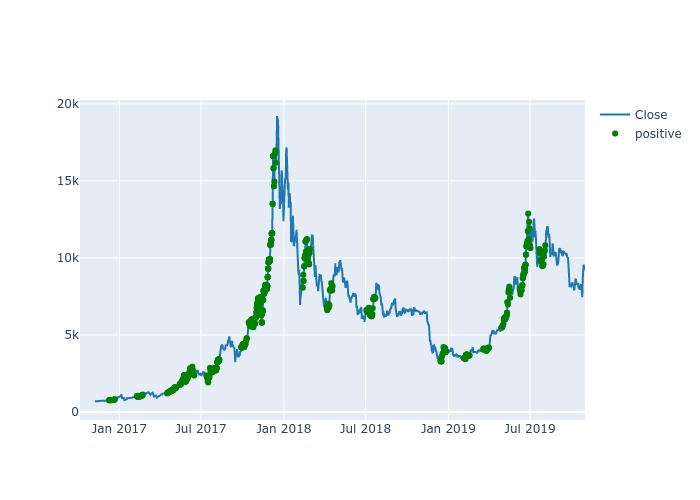
\includegraphics[width=\linewidth]{images/BTC.jpg}
      \caption{Bitcoin}
      \label{fig:bitcoin}
    \end{subfigure}
    \begin{subfigure}[b]{0.45\linewidth}
      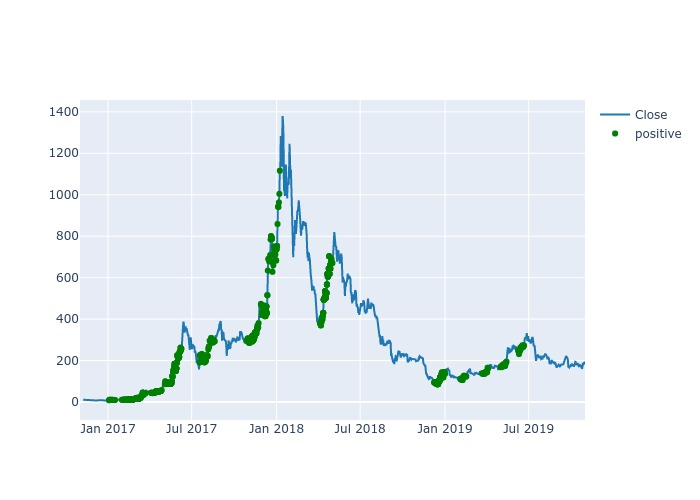
\includegraphics[width=\linewidth]{images/ETH.jpg}
      \caption{Ethereum}  
      \label{fig:ethereum}
    \end{subfigure}
    \begin{subfigure}[b]{0.45\linewidth}
        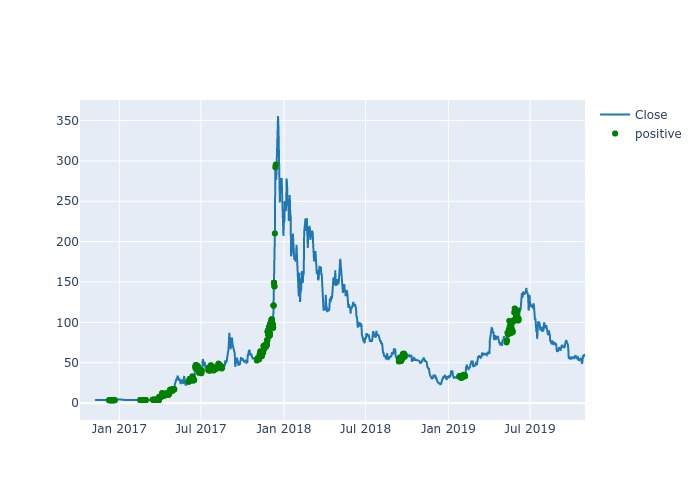
\includegraphics[width=\linewidth]{images/LTC.jpg}
        \caption{Litecoin}  
        \label{fig:litecoin}
    \end{subfigure}
    \begin{subfigure}[b]{0.45\linewidth}
        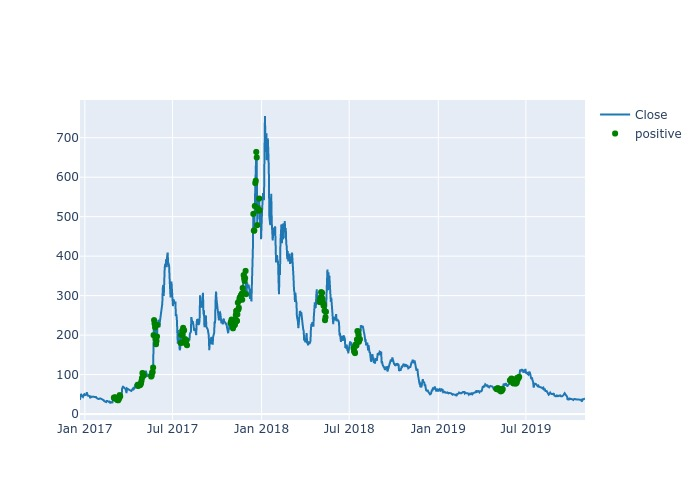
\includegraphics[width=\linewidth]{images/ZEC.jpg}
        \caption{ZCash}  
        \label{fig:zcash}
    \end{subfigure}
    \begin{subfigure}[b]{0.45\linewidth}
        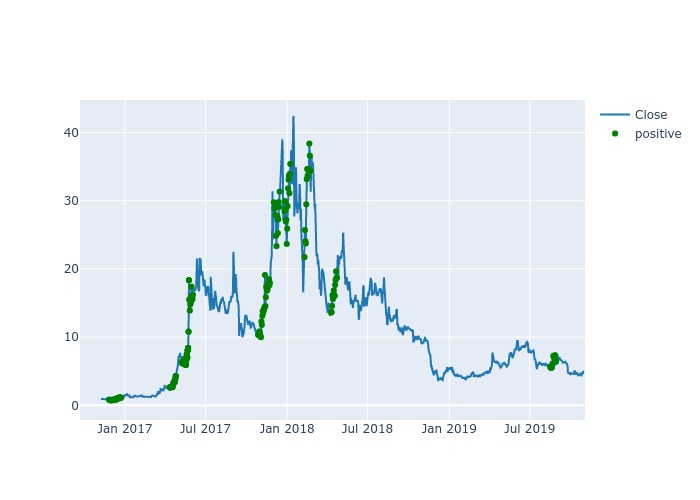
\includegraphics[width=\linewidth]{images/ETC.jpg}
        \caption{Ethereum Classic}  
        \label{fig:etc}
    \end{subfigure}
\end{figure}

\newpage
\subsection{Feature Strength}
\label{sec:feature_strength}
\begin{table}[H]
    \begin{tabular}{|l|l|l|l|l|l|}
    \hline
    \textbf{feature}                    & \textbf{ETH} & \textbf{BTC} & \textbf{ZEC} & \textbf{ETC} & \textbf{LTC} \\ \hline
    20D\_short\_volume\_mean            & 0.11         & 0.047        & 0.035        & 0.025        & 0.081        \\ \hline
    last\_price                         & 0.041        & 0.032        & 0.018        & 0.037        & 0.032        \\ \hline
    High                                & 0.04         & 0.032        & 0.015        & 0.026        & 0.037        \\ \hline
    20D\_long\_volume\_std              & 0.039        & 0.049        & 0.044        & 0.034        & 0.084        \\ \hline
    Open                                & 0.039        & 0.023        & 0.016        & 0.024        & 0.022        \\ \hline
    longshort\_ratio                    & 0.038        & 0.028        & 0.032        & 0.026        & 0.03         \\ \hline
    Low                                 & 0.036        & 0.024        & 0.015        & 0.038        & 0.03         \\ \hline
    long\_20D\_short                    & 0.035        & 0.021        & 0.041        & 0.035        & 0.038        \\ \hline
    thirty\_day\_count                  & 0.034        & 0.023        & 0.031        & 0.05         & 0.019        \\ \hline
    20D\_long\_volume\_mean             & 0.034        & 0.058        & 0.075        & 0.031        & 0.041        \\ \hline
    long                                & 0.034        & 0.036        & 0.035        & 0.048        & 0.03         \\ \hline
    short\_20D\_long                    & 0.032        & 0.052        & 0.033        & 0.026        & 0.033        \\ \hline
    20D\_short\_volume\_std             & 0.031        & 0.021        & 0.022        & 0.034        & 0.03         \\ \hline
    longshort\_volume                   & 0.03         & 0.027        & 0.029        & 0.032        & 0.019        \\ \hline
    short                               & 0.03         & 0.047        & 0.069        & 0.01         & 0.042        \\ \hline
    20D\_total\_sentiment\_mean         & 0.03         & 0.022        & 0.032        & 0.059        & 0.032        \\ \hline
    Close                               & 0.028        & 0.025        & 0.013        & 0.025        & 0.035        \\ \hline
    20D\_long\_change\_avg              & 0.023        & 0.02         & 0.023        & 0.034        & 0.021        \\ \hline
    20D\_short\_times\_above            & 0.019        & 0.014        & 0.014        & 0.022        & 0.015        \\ \hline
    volume\_from\_1\_day                & 0.016        & 0.009        & 0.018        & 0.009        & 0.009        \\ \hline
    Volume                              & 0.015        & 0.008        & 0.017        & 0.01         & 0.009        \\ \hline
    20D\_long\_times\_above             & 0.015        & 0.024        & 0.037        & 0.027        & 0.015        \\ \hline
    volume\_from\_3\_day                & 0.015        & 0.016        & 0.032        & 0.007        & 0.025        \\ \hline
    20D\_short\_change\_avg             & 0.015        & 0.019        & 0.024        & 0.053        & 0.039        \\ \hline
    volume\_from\_2\_day                & 0.014        & 0.014        & 0.016        & 0.007        & 0.017        \\ \hline
    20D\_short\_above\_avg              & 0.013        & 0.006        & 0.016        & 0.005        & 0.004        \\ \hline
    5d\_volatility                      & 0.011        & 0.012        & 0.015        & 0.009        & 0.017        \\ \hline
    20D\_long\_moving\_z\_score         & 0.011        & 0.013        & 0.022        & 0.012        & 0.006        \\ \hline
    volume\_to\_3\_day                  & 0.011        & 0.021        & 0.025        & 0.009        & 0.021        \\ \hline
    5d\_20d\_volatility\_change         & 0.01         & 0.015        & 0.008        & 0.021        & 0.005        \\ \hline
    two\_day\_change                    & 0.01         & 0.017        & 0.005        & 0.012        & 0.006        \\ \hline
    20D\_short\_moving\_z\_score        & 0.01         & 0.013        & 0.015        & 0.025        & 0.012        \\ \hline
    vol\_from\_vol\_3\_day              & 0.01         & 0.007        & 0.012        & 0.012        & 0.008        \\ \hline
    volume\_to\_2\_day                  & 0.009        & 0.014        & 0.02         & 0.005        & 0.014        \\ \hline
    20D\_short\_today\_avg\_comparision & 0.007        & 0.01         & 0.006        & 0.007        & 0.004        \\ \hline
    20D\_long\_above\_avg               & 0.007        & 0.007        & 0.007        & 0.003        & 0.003        \\ \hline
    vol\_from\_vol\_2\_day              & 0.007        & 0.005        & 0.006        & 0.005        & 0.006        \\ \hline
    volume\_change                      & 0.006        & 0.012        & 0.006        & 0.014        & 0.005        \\ \hline
    return\_vol\_3\_day                 & 0.006        & 0.01         & 0.011        & 0.015        & 0.01         \\ \hline
    three\_day\_count                   & 0.005        & 0.012        & 0.007        & 0.005        & 0.004        \\ \hline
    return\_3\_day                      & 0.005        & 0.007        & 0.006        & 0.009        & 0.005        \\ \hline
    one\_thirty\_ratio                  & 0.005        & 0.007        & 0.003        & 0.003        & 0.004        \\ \hline
    vol\_to\_vol\_3\_day                & 0.005        & 0.009        & 0.008        & 0.011        & 0.006        \\ \hline
    normalized\_mean\_sentiment         & 0.005        & 0.006        & 0.001        & 0.004        & 0.003        \\ \hline
    return\_1\_day                      & 0.005        & 0.006        & 0.004        & 0.009        & 0.004        \\ \hline
    20D\_short\_change                  & 0.004        & 0.009        & 0.004        & 0.008        & 0.005        \\ \hline
    total\_news                         & 0.004        & 0.007        & 0.001        & 0.003        & 0.002        \\ \hline
    return\_2\_day                      & 0.004        & 0.006        & 0.004        & 0.008        & 0.003        \\ \hline
    volume\_to\_1\_day                  & 0.004        & 0.009        & 0.007        & 0.007        & 0.009        \\ \hline
    return\_vol\_2\_day                 & 0.004        & 0.007        & 0.007        & 0.006        & 0.004        \\ \hline
    total\_sentiment                    & 0.004        & 0.006        & 0.002        & 0.006        & 0.003        \\ \hline
    mean\_sentiment                     & 0.004        & 0.006        & 0.001        & 0.004        & 0.003        \\ \hline
    vol\_in\_coin                       & 0.004        & 0.01         & 0.012        & 0.004        & 0.008        \\ \hline
    vol\_to\_vol\_2\_day                & 0.004        & 0.007        & 0.005        & 0.005        & 0.007        \\ \hline
    20D\_long\_today\_avg\_comparision  & 0.003        & 0.009        & 0.005        & 0.01         & 0.01         \\ \hline
    20D\_long\_change                   & 0.003        & 0.008        & 0.007        & 0.006        & 0.004        \\ \hline
    three\_thirty\_ratio                & 0.003        & 0.011        & 0.006        & 0.009        & 0.01         \\ \hline
    news\_dominance                     & 0.003        & 0.008        & 0.0          & 0.003        & 0.003        \\ \hline
\end{tabular}
\end{table}

\newpage

\subsection{Backtest Chart}
\label{sec:backtest_chart}
\begin{figure}[H]
    \centering
    \begin{subfigure}[b]{1\linewidth}
      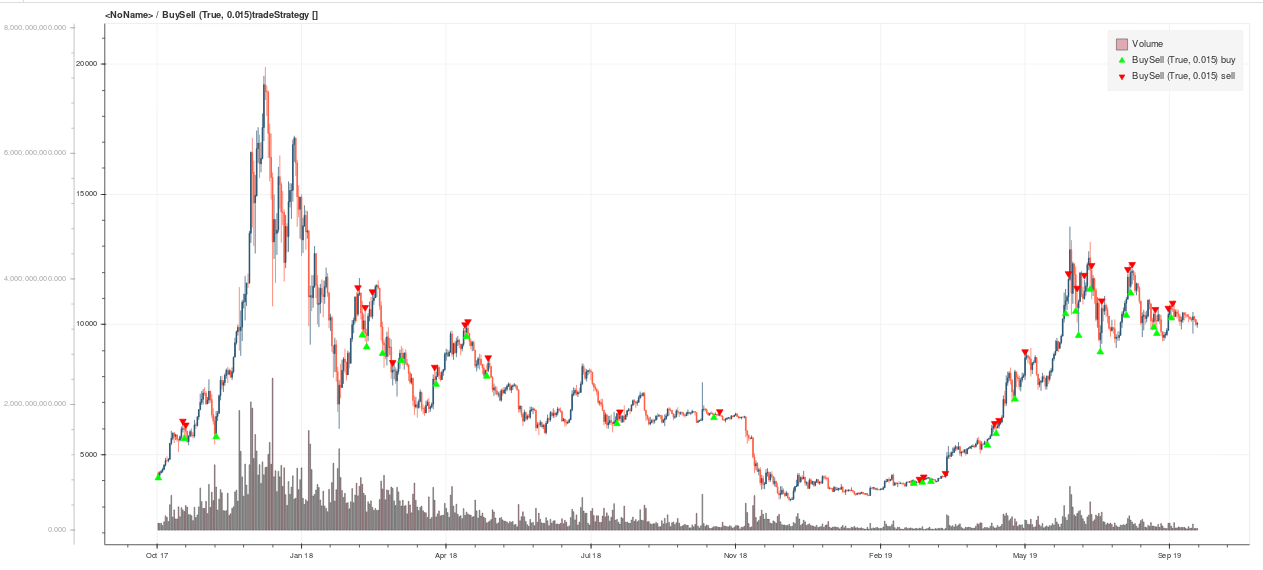
\includegraphics[width=\linewidth]{images/backtest/BTC.png}
      \caption{Bitcoin}
      \label{fig:bitcoin}
    \end{subfigure}
    \begin{subfigure}[b]{1\linewidth}
      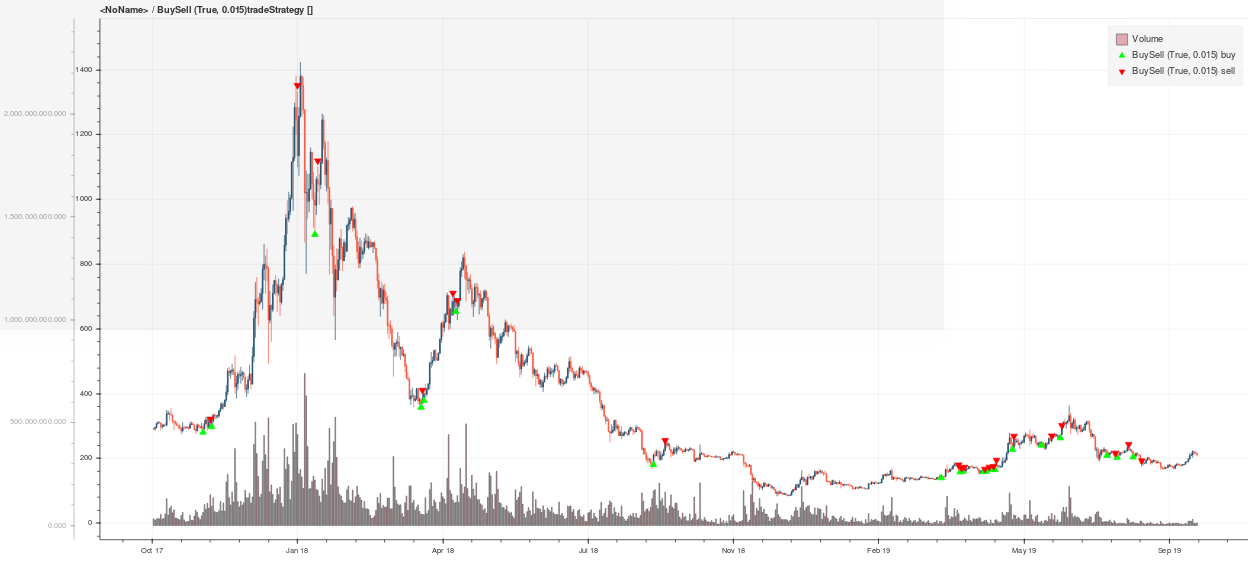
\includegraphics[width=\linewidth]{images/backtest/ETH.png}
      \caption{Ethereum}  
      \label{fig:ethereum}
    \end{subfigure}
    \newpage
\end{figure}
\begin{figure}[]\ContinuedFloat
    \centering
    \begin{subfigure}[b]{1\linewidth}
      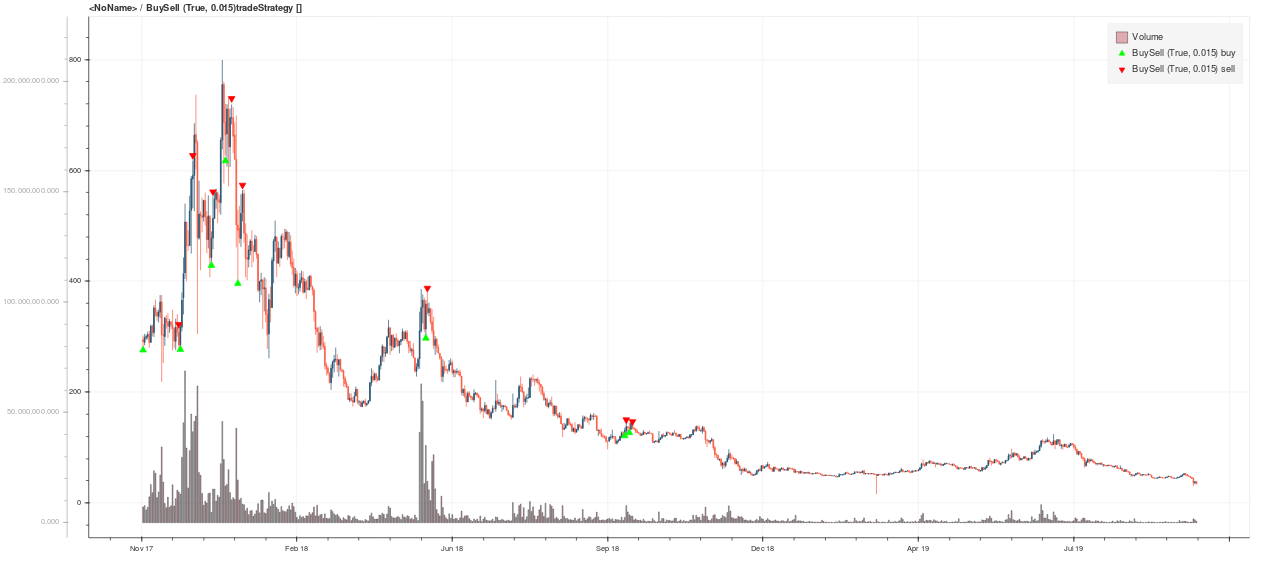
\includegraphics[width=\linewidth]{images/backtest/ZEC.png}
      \caption{ZCash}
      \label{fig:zcash}
    \end{subfigure}
    \begin{subfigure}[b]{1\linewidth}
      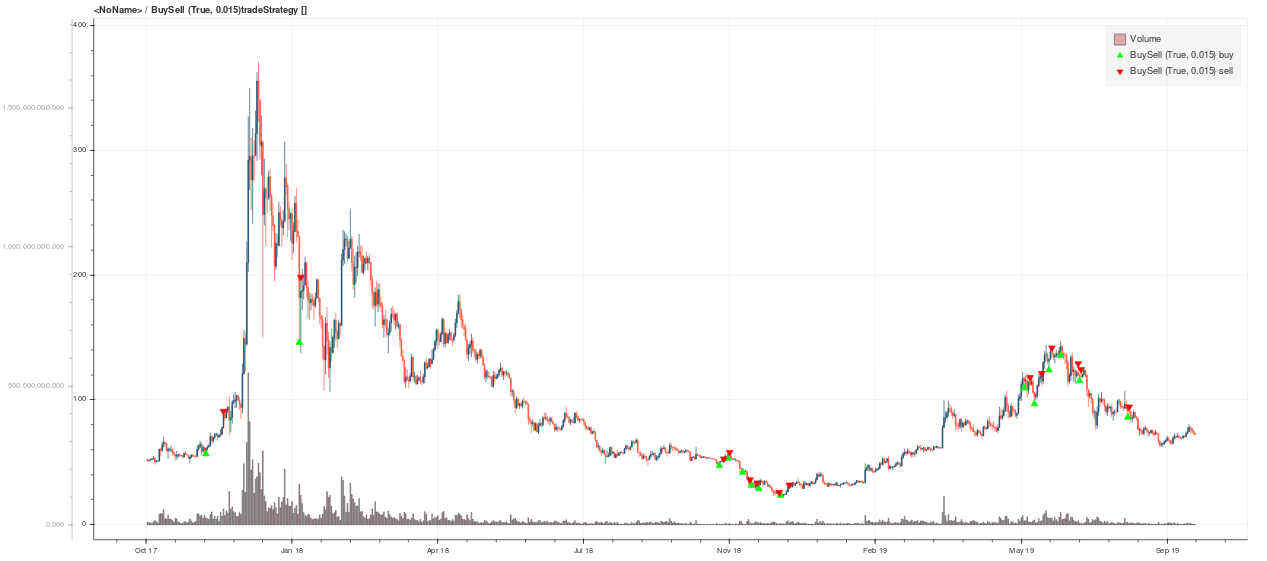
\includegraphics[width=\linewidth]{images/backtest/LTC.png}
      \caption{Litecoin}  
      \label{fig:litecoin}
    \end{subfigure}
    \newpage
\end{figure}
\begin{figure}[]\ContinuedFloat
    \centering
    \begin{subfigure}[b]{1\linewidth}
      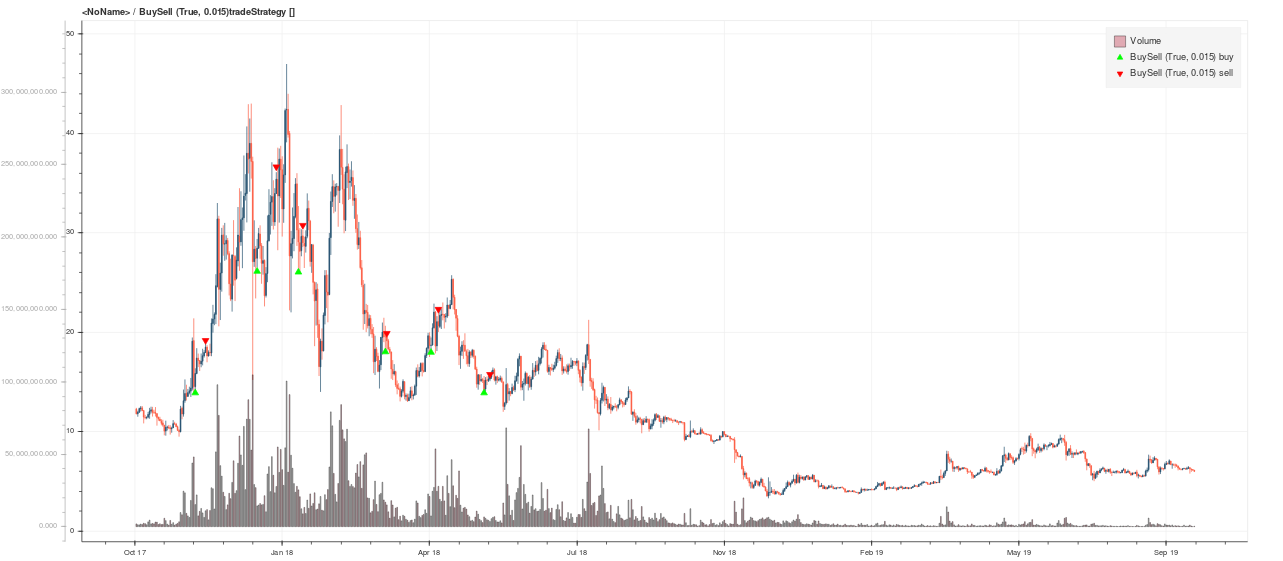
\includegraphics[width=\linewidth]{images/backtest/ETC.png}
      \caption{Ethereum Classic}
      \label{fig:etc}
    \end{subfigure}
\end{figure}

\end{document}